\documentclass[12pt,landscape,letterpaper]{article}
\usepackage{multicol,multirow}
\usepackage{graphicx}
\usepackage{ifthen}
\usepackage[landscape]{geometry}
\usepackage{booktabs}
\usepackage{fontspec}

\setsansfont{Fira Sans}
\setmonofont{Inconsolata}

\makeatother

\ifthenelse{\lengthtest { \paperwidth = 11in}}
    { \geometry{margin=0.4in} }
	{\ifthenelse{ \lengthtest{ \paperwidth = 297mm}}
		{\geometry{top=1cm,left=1cm,right=1cm,bottom=1cm} }
		{\geometry{top=1cm,left=1cm,right=1cm,bottom=1cm} }
	}
\pagestyle{empty}
\makeatletter
\renewcommand{\section}{\@startsection{section}{1}{0mm}%
                                {-4ex plus -.5ex minus -.2ex}%
                                {0.5ex plus .2ex}%x
                                {\sffamily\large}}
\renewcommand{\subsection}{\@startsection{subsection}{2}{0mm}%
                                {-4ex plus -.5ex minus -.2ex}%
                                {0.5ex plus .2ex}%
                                {\sffamily\normalsize\itshape}}

\makeatother
\setcounter{secnumdepth}{0}
\setlength{\parindent}{0pt}
\setlength{\parskip}{0pt plus 0.5ex}
% -----------------------------------------------------------------------
\usepackage{tikz}
\usepackage{float}

\begin{document}
\tikz[remember picture,overlay] \node[opacity=0.1,inner sep=0pt] at (current page.west){
\includegraphics[height=0.8\paperheight]{media/Logo.png}};
\footnotesize

\begin{center}
  {\huge\sffamily\bfseries Instruction Manual Matrixtester v1} \\
\end{center}
\setlength{\premulticols}{0pt}
\setlength{\postmulticols}{0pt}
\setlength{\multicolsep}{1pt}
\setlength{\columnsep}{1.8em}
\begin{multicols}{3}

\section{Scope of delivery}
\begin{itemize}
\item Matrixtester
\item USB Type A - Type B Cable
\end{itemize}

\section{Getting started}
This section will describe steps to be taken befor every run of testing.

\subsection{\#1 - Powering the device}

Use the cable which was included with the shipment to connect the device to a suitable USB outlet. As an alternative you could use a 5V USB power supply or a 12V round plug power supply (not included in shipment).\\

The display will lighten up for a few seconds before turning off and then on again.\\

Now the display shows the version of the device and the request to plug in a matrix in an endless loop.\\

\begin{figure}[H]
    \centering
    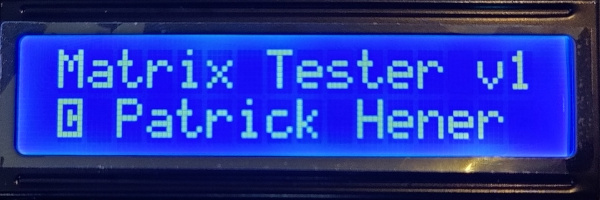
\includegraphics[width=0.2\textwidth]{media/intro-1.jpg}
\end{figure}


\begin{figure}[H]
    \centering
    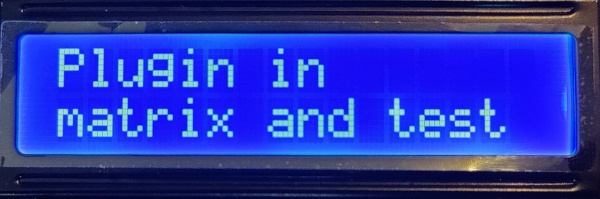
\includegraphics[width=0.2\textwidth]{media/intro-2.jpg}
\end{figure}

\subsection{\#2 Connecting the matrix}

The matrixtester exposes a pin header, where you are supposed to plugin the matrix. The pin header is marked L (for left) and R (for right) on the device case.\\

If you lay down the matrix as pictured below, your plug will be oriented left and right as labeled in the picture:

\begin{figure}[H]
    \centering
    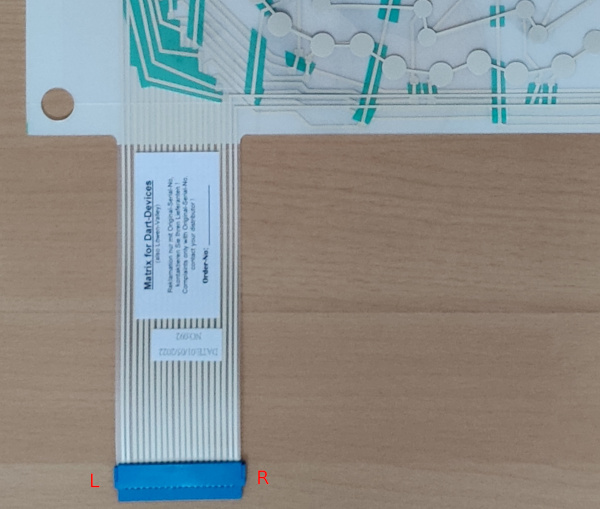
\includegraphics[width=0.2\textwidth]{media/matrix-1.jpg}
\end{figure}

The connection to the device then will be as pictured below:

\begin{figure}[H]
    \centering
    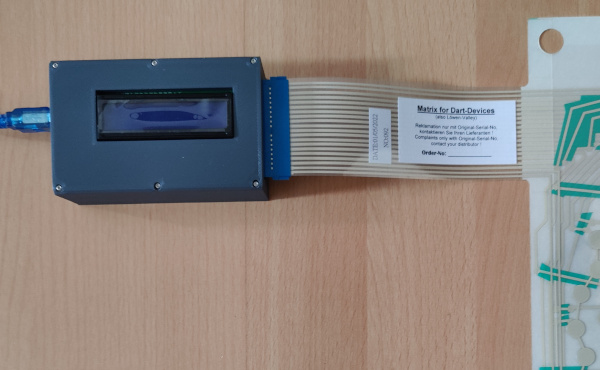
\includegraphics[width=0.2\textwidth]{media/matrix-2.jpg}
\end{figure}

\section{Testing a matrix}

To start the recognition you press and hold a trigger point of the matrix until the display shows a numerical value:

\begin{figure}[H]
    \centering
    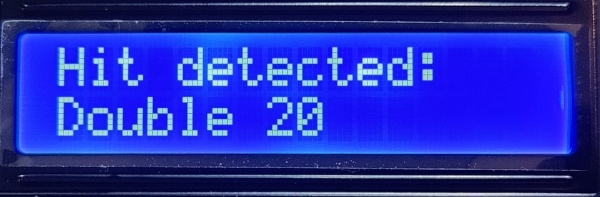
\includegraphics[width=0.2\textwidth]{media/detection-1.jpg}
\end{figure}

Then you can shortly press any other trigger point of the matrix to get the next numeric value:

\begin{figure}[H]
    \centering
    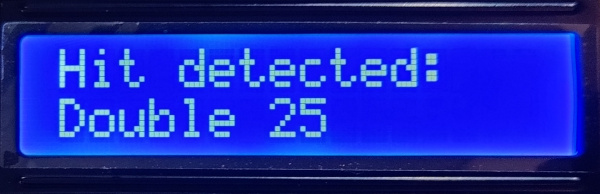
\includegraphics[width=0.2\textwidth]{media/detection-2.jpg}
\end{figure}

If you are finished with testing the matrix you can just unplug the matrix and plug back in another one. There is no need to power down the device to do so.

\vfill
{\hfill
\includegraphics[width=0.9\hsize]{media/Banner.png}\hfill}

\end{multicols}
\end{document}